%%%%%%%%%%%%%%%%%%%%%%%%%%
%%% author : Yamada. T %%%
%%% made for TH series %%%
%%%%%%%%%%%%%%%%%%%%%%%%%%

\documentclass[b5paper,10pt,fleqn] {ltjsarticle}

\usepackage[margin=10truemm]{geometry}

\usepackage{pict2e, graphicx}
\usepackage{tikz}
\usetikzlibrary{intersections,calc,arrows.meta}

\usepackage{amsmath, amssymb, amsthm}
\usepackage{ascmac}
\usepackage{comment}
\usepackage{empheq}
\usepackage[shortlabels,inline]{enumitem}
\usepackage{fancybox}
\usepackage{fancyhdr}
\usepackage{here}
\usepackage{lastpage}
\usepackage{listings, jvlisting}
\usepackage{fixdif}

\usepackage{stmaryrd}
\usepackage[listings]{tcolorbox}
%\usepackage{ascolorbox}
\usepackage{titlesec}
\usepackage{ulem}
\usepackage{url}
\usepackage{verbatim}
\usepackage{wrapfig}
\usepackage{xcolor}
\usepackage{luatexja-ruby}
\usepackage{varwidth}
\usepackage[version=3]{mhchem}
\usepackage{wrapfig}


\usepackage{physics2}
	\usephysicsmodule{ab}
	\usephysicsmodule{ab.braket}
	\usephysicsmodule{ab.legacy}
	%\usephysicsmodule{braket}
	\usephysicsmodule{diagmat}
	\usephysicsmodule{xmat}
	\usephysicsmodule{nabla.legacy}
	\usephysicsmodule{qtext.legacy}

\usepackage[ISO]{diffcoeff}
\difdef { f, s } { D }
{ op-symbol = \mathrm{D} }


\newcommand{\mctext}[1]{\mbox{\textcircled{\scriptsize{#1}}}}
\newcommand{\ctext}[1]{\textcircled{\scriptsize{#1}}}
\newcommand{\ds}{\displaystyle}
\newcommand{\comb}[2]{{}_{#1}\mathrm{C}_{#2}}
\newcommand{\hs}{\hspace}
\newcommand{\vs}{\vspace}
\newcommand{\emphvs}{\vspace{1em}\notag\\}
\newcommand{\ora}{\overrightarrow}
\newcommand{\ol}{\overline}
\newcommand{\oramr}[1]{\overrightarrow{\mathrm{#1}}}
\newcommand{\tri}{\triangle}
\newcommand{\mr}{\mathrm}
\newcommand{\mb}{\mathbb}
\newcommand{\mrvec}[1]{\overrightarrow{\mathrm{#1}}}
\newcommand{\itvec}{\overrightarrow}
\newcommand{\bs}{\boldsymbol}
\newcommand{\ra}{\rightarrow}
\newcommand{\Ra}{\Rightarrow}
\newcommand{\lra}{\longrightarrow}
\newcommand{\Lra}{\Longrightarrow}
\newcommand{\la}{\leftarrow}
\newcommand{\La}{\Leftarrow}
\newcommand{\lla}{\longleftarrow}
\newcommand{\Lla}{\Longleftarrow}
\newcommand{\lr}{\leftrightarrow}
\newcommand{\llr}{\longleftrightarrow}
\newcommand{\Llr}{\Longleftrightarrow}
\renewcommand{\deg}{{}^\circ}
\newcommand{\phbox}{\fbox{\phantom{1\hspace{2em}}}}
\newcommand{\boxnum}[1]{\fbox{\phantom{\hspace{1em}}({#1})\phantom{\hspace{1em}}}}
\newcommand{\boxkana}[1]{\fbox{\phantom{\hspace{1em}}{#1}\phantom{\hspace{1em}}}}
\newcommand{\boxkm}[2]{\fbox{\, {#1}\phantom{\hspace{0.2em}} \,  {#2}}}
\newcommand{\hzw}{\hspace{1\zw}}

\renewcommand{\baselinestretch}{1.25}
\parindent=1\zw

%TH3-3
%%東大2009第一問
\begin{document}
\noindent
\fbox{NewTH1-9} [東京大]

図1--1のように,鉛直に固定した透明な管がある.ばね定数$k$のばねの下端を管の底面に固定し,上端を質量$m$の物体1に接続する.
質量が同じく$m$の物体2を,物体1の上に固定せずにのせる.
地面上の一点Oを原点として鉛直上向きに$x$軸をとる.
ばねが自然長になっている時の物体1の$x$座標は$h$であり,重力加速度の大きさは$g$である.

なお,物体の大きさは小さく,管との摩擦や空気抵抗は無視でき,$x$方向以外の運動は考えない.
ばねの質量は無視できる.
また,管は十分長く,実験中に物体が飛び出すことはないものとする.

\begin{enumerate}[I]
  \item {\hzw}物体1と物体2を,互いに接した状態で,物体1の$x$座標が$x_\mr{A}$となる位置まで押し下げ,時刻$t = 0$に初速度0で放したところ,物体1と物体2は互いに接した状態で単振動を開始した.
  \begin{enumerate}[(1)]
    \item {\hzw}この時の,物体1の単振動の中心の$x$座標を答えよ.
    \item {\hzw}物体1と物体2の$x$方向の運動方程式をそれぞれ書け.各物体の加速度を$a_1$,$a_2$,物体1の位置を$x$,互いに及ぼす抗力の大きさを$N \ (N \geqq 0)$とせよ.
    \item {\hzw}$x_\mr{A}$の値によっては,運動中に物体1と物体2が分離することがある.図1--2はこのような場合の物体の位置の時間変化を示す.運動方程式を使って,分離の瞬間の物体1の$x$座標を求めよ.なお,図1--2では物体の大きさは無視されており,接している間の物体1と物体2の位置を1本の実線で表している.
    \item {\hzw}分離の瞬間の物体1の速度を答えよ.また,分離が起こるのは,時刻$t=0$における物体1の位置がどのような条件を満たす場合か答えよ.
  \end{enumerate}
  \item {\hzw}物体1と物体2が分離した後の運動について考える.分離後,物体1は単独で単振動する.物体2は重力のために,分離後ある時間が経過した後に必ず物体1に衝突する.分離から衝突までの時間は時刻$t = 0$における物体1の位置$x_\mr{A}$に依存する.ここで,分離から衝突までの時間が,物体1が単独で単振動する際の周期$T$に等しくなるように$x_\mr{A}$の値を設定した.衝突の時刻を$T_1$とする.
  \begin{enumerate}[(1)]
    \item {\hzw}物体1が単独で単振動する際の周期$T$を答えよ.また,物体1と物体2が衝突する瞬間(時刻$T_1$)の物体1の$x$座標を答えよ.
    \item {\hzw}分離の瞬間の物体2の速度を$V$とする.分離から衝突までの時間が$T$となるための$V$の満たす式を書け.
    \item {\hzw}物体1と物体2の間のはねかえり係数は1であるとし,時刻$T_1$における衝突以降の運動を考える.物体1と物体2が,$T_1$以降に再び接触する時刻$T_2$と,その時の物体1の$x$座標を答えよ.また,時刻$t=0$から$2T_1$までの間で,横軸を時刻,縦軸を物体の位置とするグラフの概形を描け.物体の大きさは無視し,物体1と物体2が接した状態で運動している部分は実線,分離している部分は点線を用いよ.なお,縦軸,横軸共に,値や式を記入する必要はない.
    \item {\hzw}この場合の$x_\mr{A}$を$h$,$m$,$k$,$g$を用いて表せ.
  \end{enumerate}
\end{enumerate}

\begin{figure}[H]
  \centering
  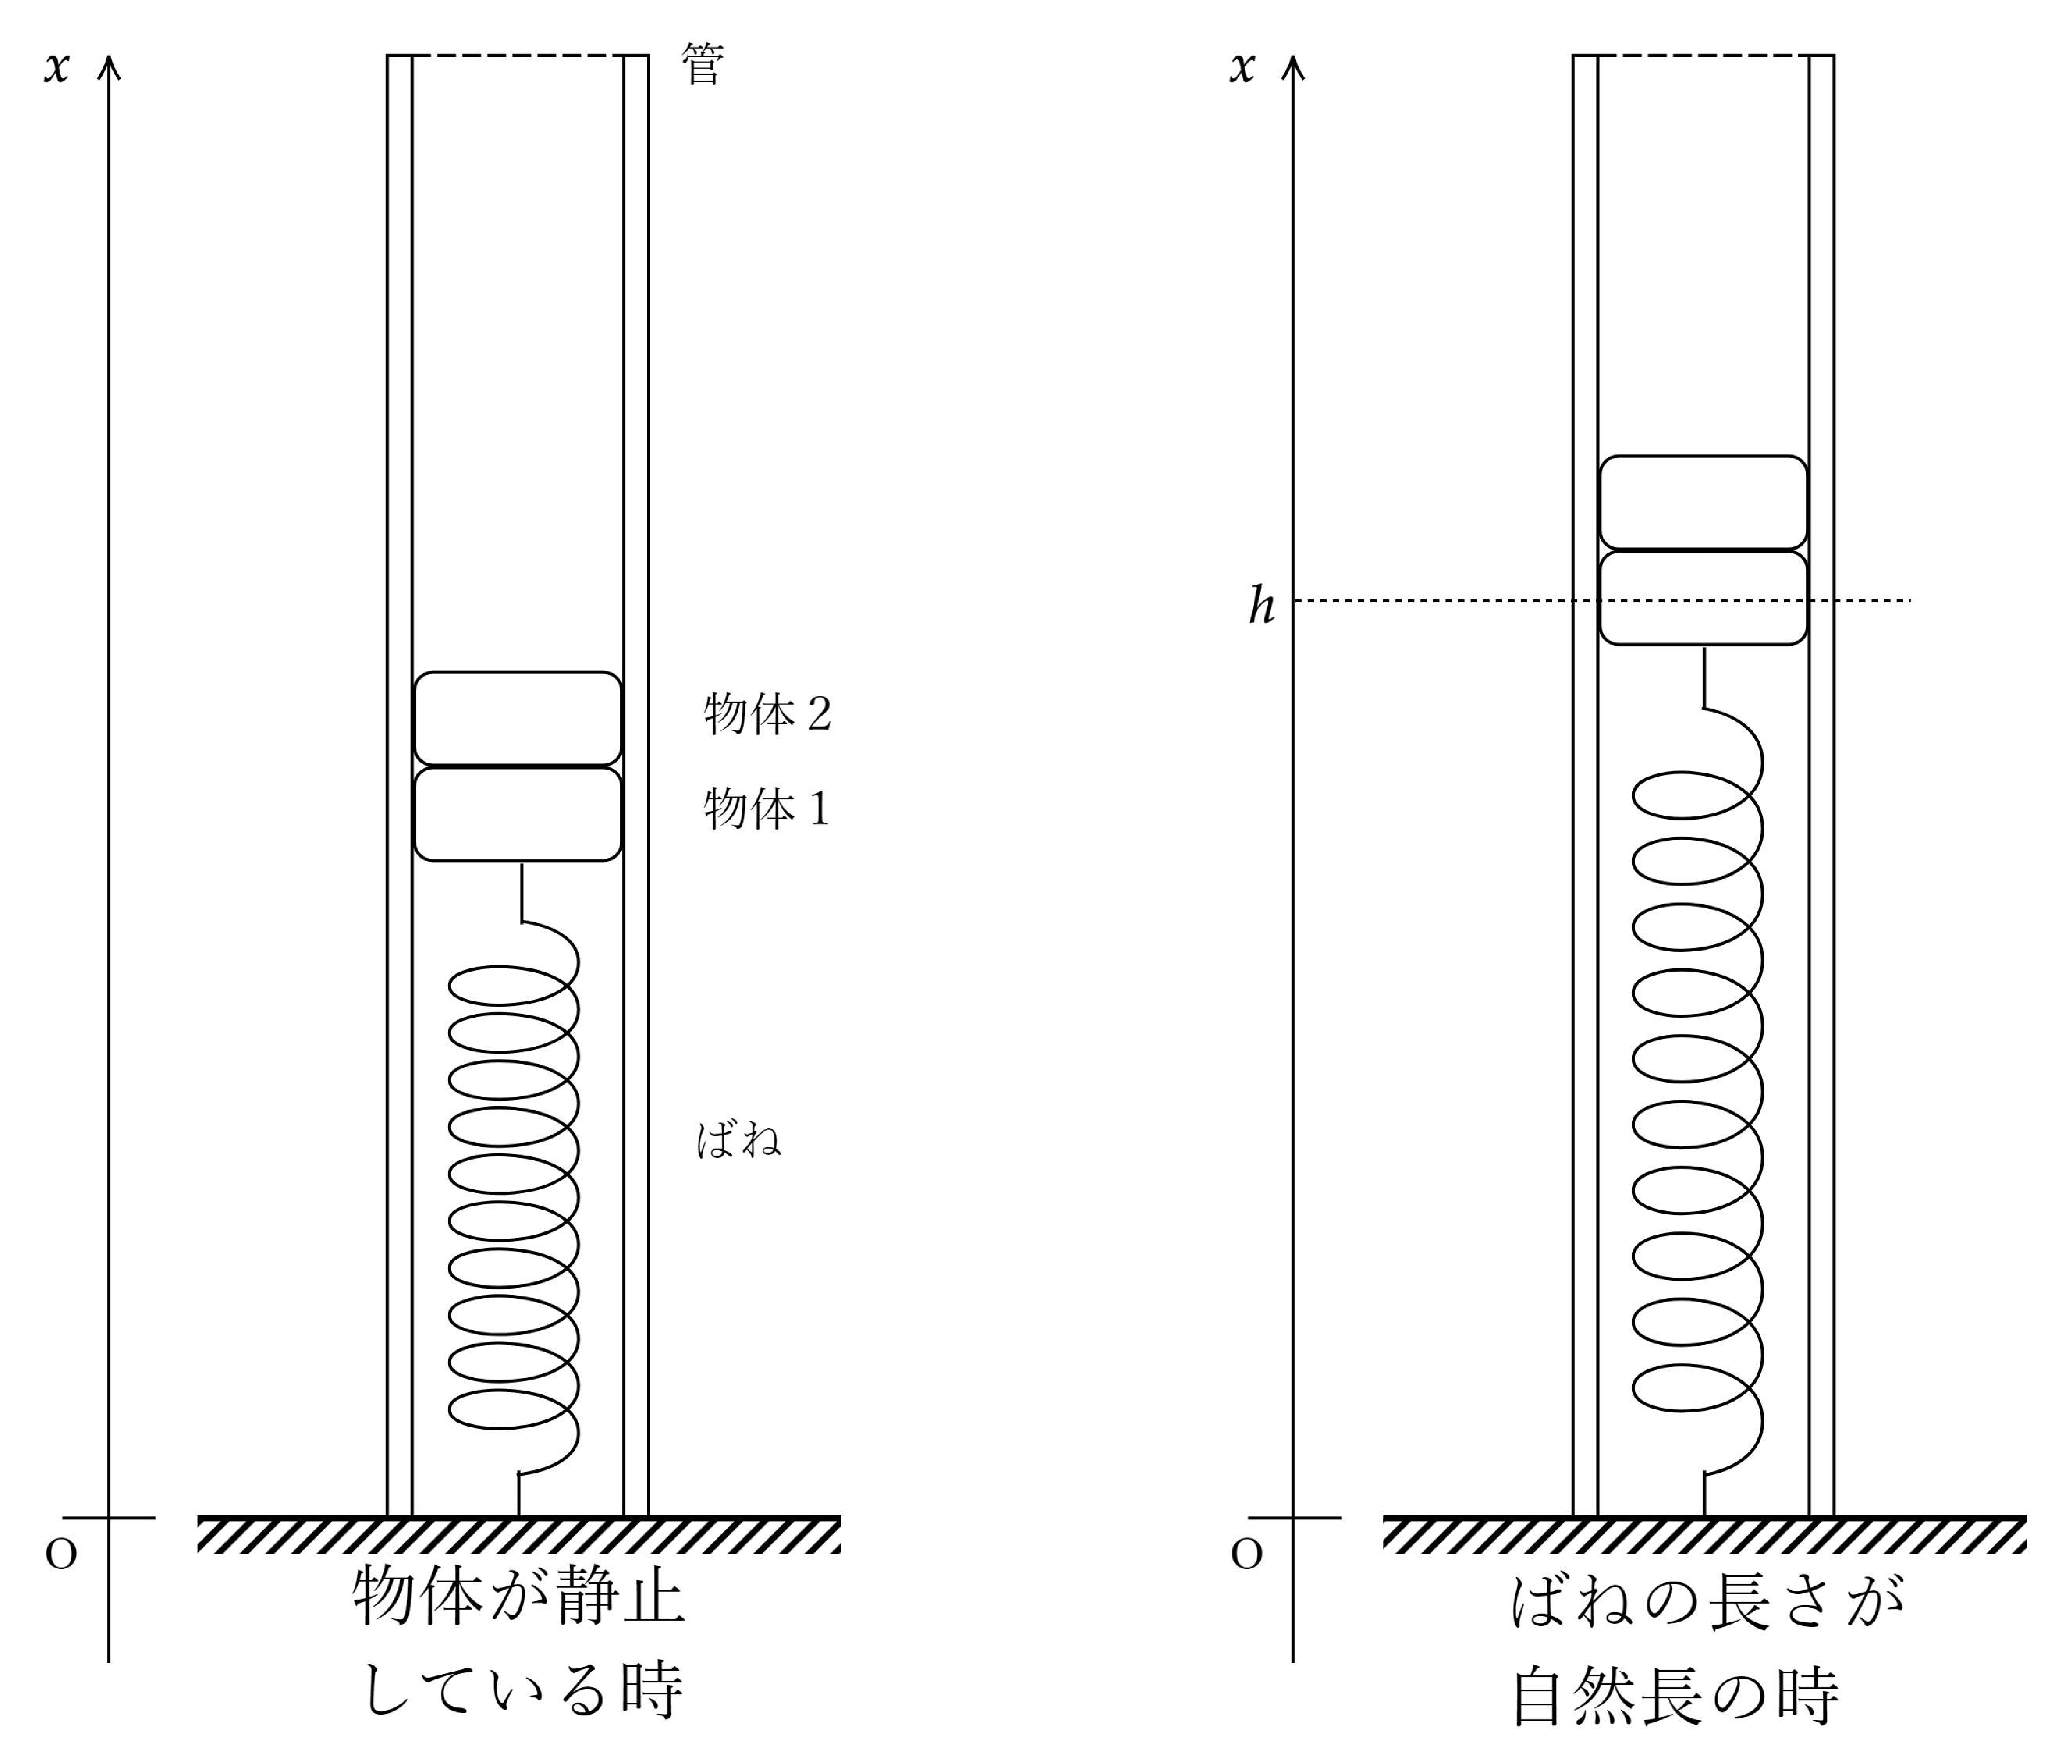
\includegraphics[width=10cm]{fig/fig_1_9_1.pdf}

  図1--1
\end{figure}

\end{document}